% Appendix C source fragment. Do not input this file into the six-page paper.
% The overall portfolio wrapper must load pdfpages and booktabs, create the
% blank Appendix C title page, establish C.1/C.2/... page numbering, and define
% the optional imported-page and content-page hooks below.
\providecommand{\PortfolioImportedPageCommand}{}
\providecommand{\PortfolioAppendixPageStyle}{}
\providecommand{\PortfolioContentPageCommand}{}

% C.1 is the complete approved plan. addtotoc records the subsection without
% placing new material over the original first page.
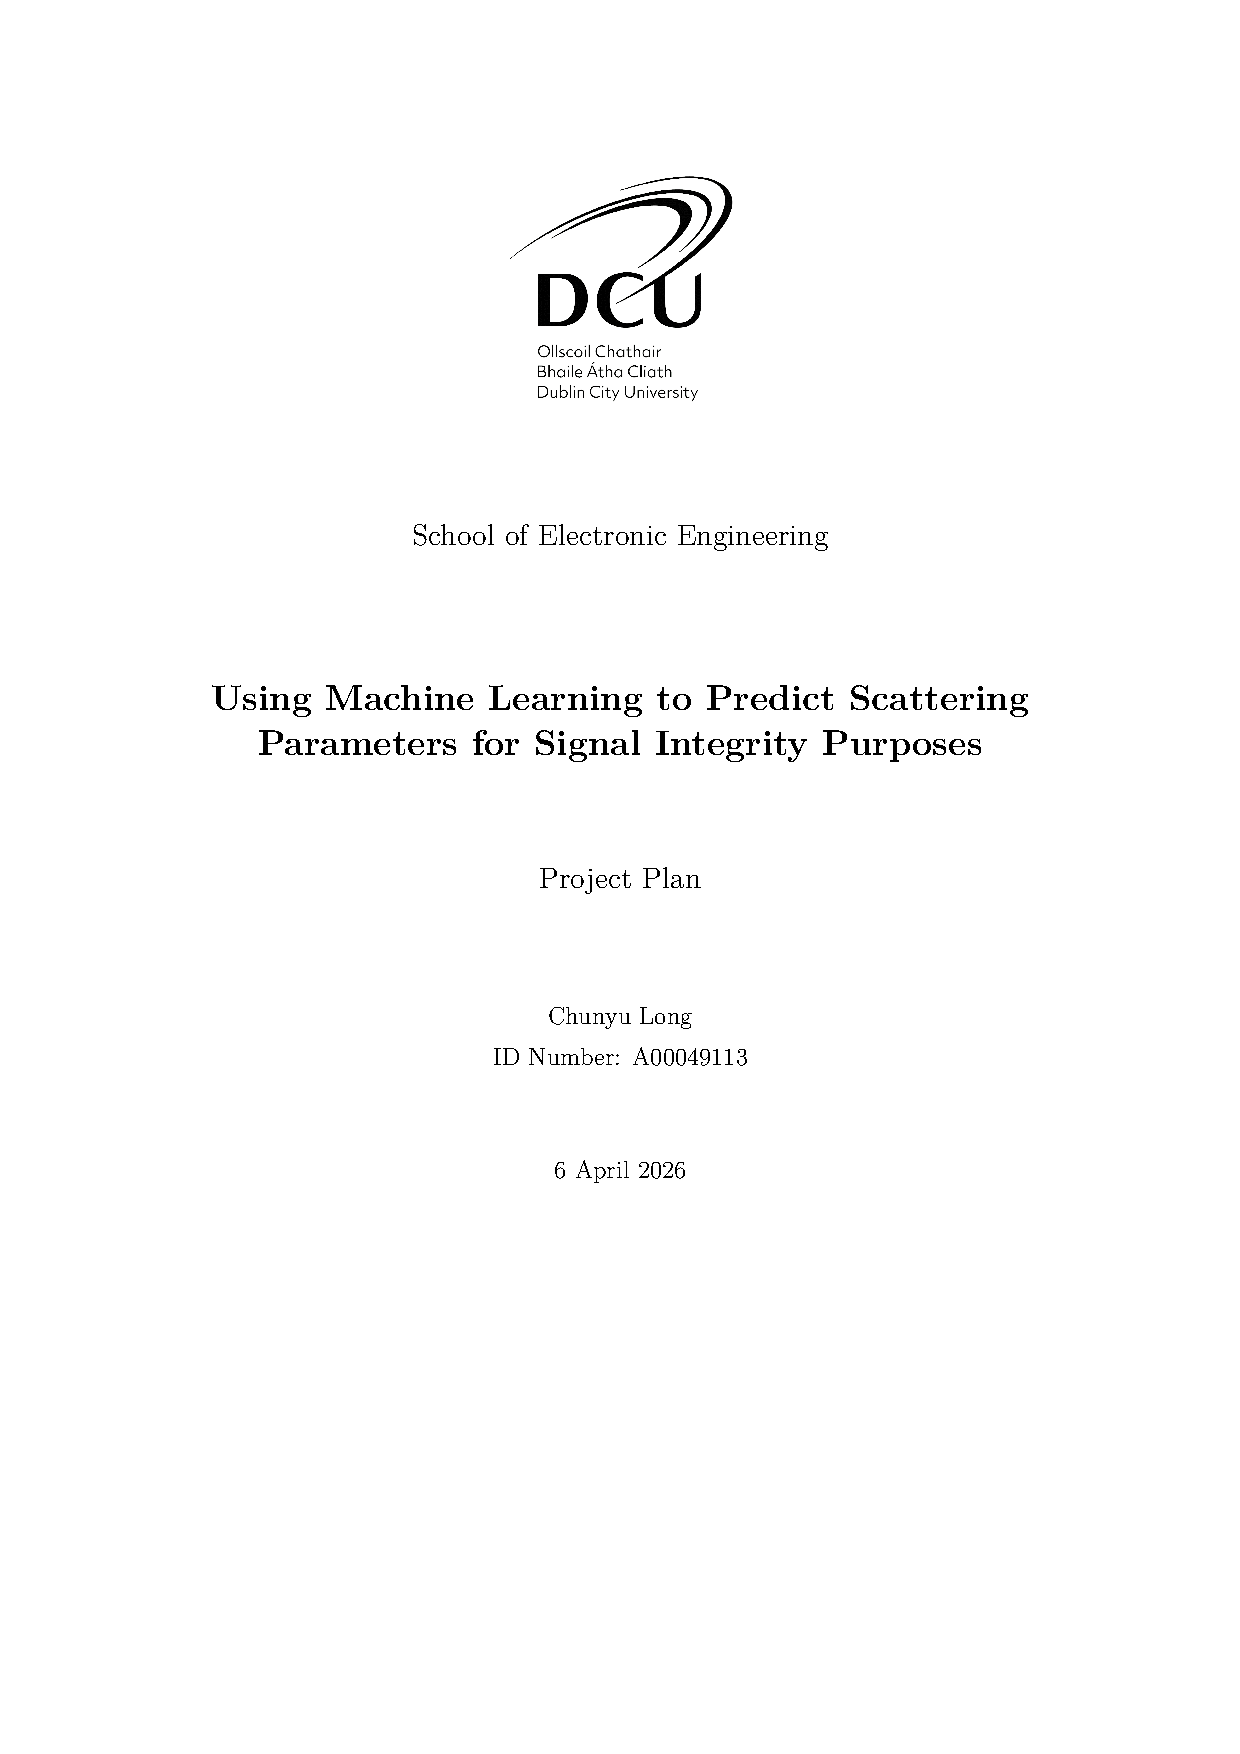
\includepdf[
    pages=-,
    fitpaper=true,
    pagecommand={\PortfolioImportedPageCommand},
    addtotoc={1,subsection,2,{C.1 Original Approved Plan},app:c-original-plan}
]{documents/ProjectPlan_A00049113_v4.0.pdf}

% The audit tables use the full page width for legibility. Return to two
% columns for the prose-based key-reference assessment in C.5.
\onecolumn
\PortfolioAppendixPageStyle
\PortfolioContentPageCommand
\phantomsection
\addcontentsline{toc}{subsection}{C.2 Progress and Key Milestones}
\subsection*{C.2 Progress and Key Milestones}
\label{app:c-progress}

The previous pages contain the complete approved EEN1101 project plan. The copy stored
in this portfolio is identical to the supplied PDF. Its SHA-256 digest is
\texttt{c6810b5da9e3a92a5a2417b596562a0d}\allowbreak
\texttt{c4d890c90e77b30b2d617e6ea173665e}.
Table~\ref{tab:appendix-c-progress} shows what was actually completed at each
planned stage. Dates in the selected run identifiers refer to the final saved
artifacts. They should not be read as a complete timeline of the exploratory
work.

In the evidence locations below, NB01 through NB08 identify the numbered
Jupyter notebooks in the submitted project repository. Appendix F maps each
label to its filename and purpose.

\begin{table}[!htbp]
    \caption{Progress and key milestones against the approved workplan.}
    \label{tab:appendix-c-progress}
    \centering
    \scriptsize
    \begin{tabular}{@{}p{0.16\textwidth}p{0.48\textwidth}
                         p{0.27\textwidth}@{}}
        \toprule
        Approved phase & What was completed & Evidence location \\
        \midrule
        Weeks 1--2:
        data pipeline
          & Linked 7,030 ten-parameter designs to complex 12-port Touchstone
            responses at 200 frequencies. All frequencies from a given design
            stayed in the same train, validation or test split. The resulting
            split contained 4,218/1,406/1,406 designs. Preprocessing was fitted
            on training data only.
          & Paper Section III; Appendix D, Shared Data and Leakage Controls;
            NB01 dataset analysis and NB02 preprocessing artifacts. \\
        Weeks 3--4:
        baselines
          & Built scalar and vector Ridge models, a powers-only Polynomial
            Ridge model and a Random Forest. Scalar Ridge achieved a test MAE
            of 7.5051~dB, compared with 12.3535~dB for the pooled global mean.
            However, it did not improve on the stronger 7.4254~dB
            frequency-dependent mean curve.
          & Paper Table I; Appendix E, Tables V--VII; NB03 selected runs. \\
        Weeks 3--6:
        point-wise neural exploration
          & Built two multilayer perceptrons with the common six-path interface.
            One used the original inputs. The other used a fifth-degree,
            powers-only expansion. Across the selected configurations, these
            models did not consistently reduce $IL_{7,1}$ error.
          & Paper Sections III--V; NB04 selected runs; Appendix D model
            descriptions and NB08 diagrams; Appendix E selected-run record. \\
        Weeks 5--7:
        whole-curve model
          & Built a model that maps one design to six curves at 200 frequencies.
            It uses a compact transposed-convolution decoder, fixed Fourier
            frequency coordinates and a curve-aware loss. The selected model
            achieved a test $IL_{7,1}$ MAE of 7.3883~dB.
          & Paper Sections III--V; Appendix D, Whole-Curve Neural Model;
            Appendix E paired comparisons; NB05 selected run. \\
        Weeks 6--9:
        complete matrix and diagnostics
          & Built a design-conditioned model for the reciprocal complex 12-port
            response. Its test complex MAE/NRMSE was 0.0686/0.7889. The
            training-mean matrix gave 0.0804/0.8343 on the same task.
            Reciprocity is exact by construction. Passivity and finite-band
            causality were checked after training.
          & Paper Sections III--V; Appendix D, Reciprocal Complete-Matrix
            Neural Model; Appendix E, Tables VIII--IX; NB06 selected run. \\
        Week 9:
        parameter study
          & The planned controlled sweep of every physical parameter was not
            completed. The final work therefore makes no parameter-sensitivity
            claim.
          & Paper limitations and future work; Tables
            \ref{tab:appendix-c-changes} and
            \ref{tab:appendix-c-objectives}. \\
        Final evaluation and
        portfolio
          & NB07 recomputed the selected metrics and produced the common-target
            and same-task comparisons. It also exported the physical
            diagnostics. The six-page paper was completed during the
            contingency period. NB08 and Appendices D--E provide the detailed
            implementation and testing record.
          & Paper; Appendices D--E; NB07--NB08; portfolio evidence exports. \\
        \bottomrule
    \end{tabular}
\end{table}

\clearpage
\PortfolioContentPageCommand
\phantomsection
\addcontentsline{toc}{subsection}{C.3 Major Changes to Scope or Methodology}
\subsection*{C.3 Major Changes to Scope or Methodology}
\label{app:c-changes}

Table~\ref{tab:appendix-c-changes} compares the approved method with the work
that was ultimately carried out. It also separates method changes from
objectives that were not completed. I use the label \emph{retrospective} when
no written approval or decision record was available from the time. I do not
describe a change as supervisor-approved unless written evidence confirms it.

\begin{table}[!htbp]
    \caption{Major method changes, reasons and consequences.}
    \label{tab:appendix-c-changes}
    \centering
    \scriptsize
    \begin{tabular}{@{}p{0.20\textwidth}p{0.27\textwidth}
                         p{0.25\textwidth}p{0.20\textwidth}@{}}
        \toprule
        Approved intent & What changed & Reason and evidence
                        & Consequence \\
        \midrule
        Row-wise input $[\mathbf u,f]$ with $2m^2$ real outputs at each
        design--frequency sample
          & The final model takes one design as input and generates the complete
            fixed 200-point response in one pass. It predicts 78 unique complex
            upper-triangle entries as 156 real channels.
          & \emph{Retrospective:} whole-grid prediction keeps the broadband
            context. Predicting only the upper triangle avoids learning
            reciprocal duplicates. The saved architecture and output contract
            confirm this change.
          & The complete-matrix objective was retained, but the approved
            formulation was not followed exactly. \\
        Complete matrix plus physical consistency
          & The predicted upper triangle is mirrored into the lower triangle.
          & The selected interconnect is passive and reciprocal. Reciprocity
            can therefore be built into the output structure, rather than
            learned twice from duplicate entries.
          & The prediction reciprocity residual is zero by construction. This
            structure does not enforce passivity or causality. \\
        Passivity and causality enforcement with a constrained/unconstrained
        comparison
          & Passivity and a finite-positive-band causality residual were checked
            after training. The selected loss gave zero weight to passivity and
            contained no causality term. A matched enforcement ablation was not
            completed.
          & \emph{Retrospective:} no passivity violation was found in the
            281,200 sampled test matrices. The selected model also did not show
            the non-physical negative insertion loss reported by Chen and Tan.
            With the time remaining, priority was given to complete-matrix
            prediction, diagnostics and a traceable evidence package.
          & Only reciprocity is guaranteed. Passivity is an observation on the
            sampled grid, while the finite-band causality result is a
            diagnostic. The planned enforcement and ablation remain unmet. \\
        Controlled variation of every physical parameter
          & The final controlled one-factor-at-a-time sweep was not completed.
          & \emph{Retrospective:} the remaining schedule was used to implement
            and validate the complete-matrix model. Completing the evidence
            package also took priority.
          & The effects on selected S-parameters, insertion loss, return loss
            and crosstalk were not established. \\
        Matrix MAE and RMSE as principal matrix errors
          & Complex MAE and complex NRMSE became the main matrix metrics. The
            common insertion-loss comparison still uses dB MAE and RMSE.
          & NRMSE relates the error to target energy. This is useful when matrix
            entries have different scales. Appendix E defines both metric
            domains.
          & The emphasis changed from RMSE to NRMSE for the complex matrix.
            Dimensionless complex errors remain separate from dB errors. \\
        Evaluation on unseen held-out data
          & Test designs were excluded from fitting. However, NB03--NB06
            inspected test results during development.
          & The progressive notebooks used test comparisons while the modelling
            path was still being developed.
          & The results are retrospective evidence on designs held out from
            fitting. They are not an untouched confirmatory test. \\
        Reduced repeated-simulation cost
          & Model inference time was recorded, but there was no matched timing
            measurement for electromagnetic simulation.
          & A comparable simulation run was not measured under a declared
            timing protocol.
          & The evidence does not support a simulation speed-up or cost-reduction
            claim. \\
        \bottomrule
    \end{tabular}
\end{table}

Several items remained intentionally outside the approved scope. These were
inverse design or geometry optimisation, a universal model spanning all
database topologies, production electronic-design-automation deployment, and
industrial replacement of electromagnetic simulation. They are not failed
objectives. The paper discusses cross-topology modelling only as future work.

\clearpage
\PortfolioContentPageCommand
\phantomsection
\addcontentsline{toc}{subsection}{C.4 Achievements Against Plan}
\subsection*{C.4 Achievements Against Plan}
\label{app:c-achievements}

Table~\ref{tab:appendix-c-objectives} gives one final status for each approved
objective or research-question component. ``Met with qualification'' means that
the core work was completed, but the evidence needs careful interpretation.
This applies when no acceptance threshold was set in advance or when a stronger
later check gives a more cautious result.

\begin{table}[!htbp]
    \caption{Approved objectives, final status and supporting evidence.}
    \label{tab:appendix-c-objectives}
    \centering
    \scriptsize
    \begin{tabular}{@{}p{0.24\textwidth}p{0.14\textwidth}
                         p{0.35\textwidth}p{0.18\textwidth}@{}}
        \toprule
        Approved objective or criterion & Status & Final evidence
                                         & Consequence \\
        \midrule
        Reproducible parameter/Touchstone pipeline by Week 2
          & Met, subject to final package audit
          & The pipeline contains 7,030 aligned designs. Split identifiers,
            training-only transforms, selected-run manifests and executable
            notebooks were saved.
          & I describe the workflow as ``documented and version-controlled''
            until Appendix F passes its clean-environment and accessibility
            audit. \\
        Baselines validate parsing, scaling, design splits and metrics by
        Week 3
          & Met with qualification
          & Scalar Ridge validation/test MAE was 7.3237/7.5051~dB. Its RMSE was
            10.8112/12.3342~dB. Test MAE improved on the 12.3535~dB pooled
            global mean, but not on the 7.4254~dB mean curve.
          & The baseline passes the specified global-mean comparison. The
            stronger frequency-dependent reference leads to a more cautious
            interpretation. \\
        Stable broadband neural prediction of the complete S-matrix by Week 6
          & Met with method change
          & Full-matrix test complex MAE/NRMSE was 0.0686/0.7889, compared with
            0.0804/0.8343 for the same-task mean matrix. Representative
            reflection and crosstalk responses were retained.
          & The approved row-wise implementation was replaced by a reciprocal
            design-to-grid formulation. \\
        Reproduce main broadband trends on held-out designs
          & Partly met
          & Aggregate errors and representative complex curves show that the
            main trends were reproduced for sampled designs. Confidence is
            limited by one selected seed and development-time test exposure.
          & The test evidence is not untouched. It also does not establish
            universal generalisation. \\
        Enforce passivity and causality and compare constrained/unconstrained
        variants by Week 8
          & Unmet
          & The reciprocity residual was 0. There were 0 passivity violations
            in 281,200 predicted matrices, and the maximum singular value was
            0.9141. The test prediction/truth finite-band causality residual was
            0.4812/0.3173. No enforcement ablation was completed.
          & These results are diagnostics. Passivity on the sampled test grid
            is not a global guarantee. \\
        Vary every physical parameter with others controlled by Week 9
          & Unmet
          & No final one-factor-at-a-time study was produced. The planned
            insertion-loss, return-loss and crosstalk analysis is also absent.
          & This remains evidence-led future work. No sensitivity claim is
            made. \\
        Final comparison with relevant broadband methods
          & Partly met
          & Paper Sections II and V compare target scope, broadband interface,
            complex representation and physical mechanisms with the five key
            works assessed in C.5.
          & The comparison remains qualitative where datasets or metrics
            differ. Missing enforcement and parameter evidence are stated
            directly. \\
        Accuracy sufficient for signal-integrity decisions
          & Not established
          & Numerical error was quantified. However, no downstream decision,
            engineering tolerance or acceptance threshold was defined.
          & The evidence does not establish task-level sufficiency or industrial
            usefulness. \\
        Reduce repeated electromagnetic-simulation cost
          & Not established
          & No matched simulation timing baseline was collected.
          & Inference timing alone cannot support a simulation speed-up claim. \\
        \bottomrule
    \end{tabular}
\end{table}

Overall, the approved composite research question was only partly answered.
The project produced a design-conditioned approximation of the complete
reciprocal complex response for one topology. It also quantified prediction
error and physical behaviour on the sampled test grid. The work did not
establish task-specific signal-integrity sufficiency. It also did not complete
passivity or causality enforcement, the controlled parameter study, or a
comparison of cost with electromagnetic simulation.

\twocolumn
\PortfolioAppendixPageStyle
\PortfolioContentPageCommand
\phantomsection
\addcontentsline{toc}{subsection}{C.5 Key References for Detailed Assessment}
\subsection*{C.5 Key References for Detailed Assessment}
\label{app:c-key-references}

These five sources provide the main foundation for the dataset, broadband
representation, physical-validity motivation, complex prediction and multi-port
comparison. Their bracketed numbers match the current six-page paper. If the
paper's bibliography order changes, these labels must be updated before
submission.

\subsubsection*{Paper reference [1] --- Schierholz et al.}
M. Schierholz, A. S\'{a}nchez-Mas\'{i}s, A. Carmona-Cruz, X. Duan, K. Roy,
C. Yang, R. Rimolo-Donadio, and C. Schuster, ``SI/PI-Database of PCB-Based
Interconnects for Machine Learning Applications,'' \emph{IEEE Access}, vol. 9,
pp. 34423--34432, 2021, doi: 10.1109/ACCESS.2021.3061788.

Schierholz \textit{et al.} introduce the open PCB-interconnect database used in
this project. They also demonstrate neural prediction of selected S-parameter
magnitude and phase. A key strength is the public pairing of parameterised
geometries with simulated Touchstone responses. The authors report lower
accuracy for electrically longer, more frequency-dependent links. This finding
is directly relevant to the selected topology. Their study focuses on selected
responses rather than a design-conditioned complete complex 12-port matrix.
This project uses one of their datasets and keeps designs separate across the
data splits. It extends prediction to the complete matrix, but remains limited
to one topology.

\subsubsection*{Paper reference [3] --- Torun et al.}
H. M. Torun, H. Yu, N. Dasari, V. C. K. Chekuri, A. Singh, J. Kim, S. K. Lim,
S. Mukhopadhyay, and M. Swaminathan, ``A Spectral Convolutional Net for
Co-Optimization of Integrated Voltage Regulators and Embedded Inductors,'' in
\emph{Proc. IEEE/ACM Int. Conf. Computer-Aided Design}, 2019, pp. 1--8,
doi: 10.1109/ICCAD45719.2019.8942109.

Torun \textit{et al.} propose a spectral transposed-convolutional network. It
generates an entire frequency response instead of treating each frequency
independently. The architecture uses local spectral structure and is well
suited to broadband outputs. However, its application and targets differ from
the 12-port PCB problem. It also does not guarantee passivity or causality. This
project adapts the transposed-convolution idea to six insertion-loss curves. It
adds fixed frequency coordinates and a curve-aware loss. The resulting model is
described as S-TCNN-style, not as an exact reproduction.

\subsubsection*{Paper reference [4] --- Chen and Tan}
L. Chen and L. Tan, ``Physics-Enforced Modeling for Insertion Loss of
Transmission Lines by Deep Neural Networks,'' in \emph{Proc. 2021 IEEE
Asia-Pacific Microwave Conf.}, 2021, pp. 276--278,
doi: 10.1109/APMC52720.2021.9661782.

Chen and Tan show that an unconstrained neural model can produce non-physical
negative insertion loss. They add physical enforcement to address this
behaviour. Their study clearly shows why numerical error alone is not enough
for a signal-integrity surrogate. However, it considers a selected insertion-
loss response rather than a complete complex multi-port matrix. In this
project, their result motivates the physical diagnostics. The selected
full-matrix predictions did not show the reported behaviour on the sampled test
grid, but the enforcement experiment was not reproduced.

\subsubsection*{Paper reference [5] --- Akinwande et al.}
O. Akinwande, S. Erdogan, R. Kumar, and M. Swaminathan, ``Surrogate Modeling
With Complex-Valued Neural Nets for Signal Integrity Applications,''
\emph{IEEE Trans. Microwave Theory Tech.}, vol. 72, no. 1, pp. 478--489,
Jan. 2024, doi: 10.1109/TMTT.2023.3319835.

Akinwande \textit{et al.} predict broadband complex $S_{11}$ and $S_{21}$ with
a complex-valued network. Their work combines phase-bearing responses with
passivity and causality considerations. However, the evaluated output is a
selected subset rather than every entry in a high-port-count matrix. This
project also preserves real and imaginary information. It uses paired
real-valued channels and predicts the complete reciprocal matrix. Only
reciprocity is enforced; passivity and causality remain diagnostics.

\subsubsection*{Paper reference [6] --- Karahan et al.}
E. A. Karahan, Z. Liu, A. Gupta, Z. Shao, J. Zhou, U. Khankhoje, and
K. Sengupta, ``Deep-Learning Enabled Generalized Inverse Design of Multi-Port
Radio-Frequency and Sub-Terahertz Passives and Integrated Circuits,''
\emph{Nature Communications}, vol. 15, art. 10734, 2024,
doi: 10.1038/s41467-024-54178-1.

Karahan \textit{et al.} demonstrate deep-learning models for complex multi-port
responses and inverse design across radio-frequency and sub-terahertz
structures. Their broad multi-port scope is important because it shows that
complex multi-port learning is not new by itself. However, their structures,
datasets, inverse-design aim and evaluation protocol differ from this PCB
interconnect problem. The present project has a narrower aim. It is a
forward-only, topology-specific study of the complete reciprocal broadband
12-port response. For this reason, no cross-paper numerical ranking is made.
